\documentclass[12pt]{article}
\usepackage{sbc-template,amssymb,amsmath} 
\usepackage{times}
\usepackage{amsmath}
\usepackage{microtype}
\usepackage{amsthm}
\usepackage{url}
\usepackage[utf8x]{inputenc}
\usepackage[T1]{fontenc}
\usepackage{color}
\usepackage{subfig}
\usepackage{mathptmx} 
\usepackage[ruled]{algorithm2e}
\usepackage[pdftex,colorlinks=false,bookmarksnumbered,pdfstartview=XYZ]{hyperref}
\usepackage{graphicx} % for compatible graphics with hyperref
\usepackage[figure,table]{hypcap} % corrects the hyper-anchor of figures/tables


\newcounter{notecounter}
\newcommand{\nota}[1]{\addtocounter{notecounter}{1}{\textcolor{red}{[nota
      \arabic{notecounter}: #1]}}}

\title{Functional Harmonic Analysis and Computational Musicology in
  Rameau}

\author{Alexandre Tachard Passos\inst{1}, Marcos Sampaio\inst{2},
  Pedro Kröger\inst{2}, Givaldo de Cidra\inst{2}}

\address{Instituto de Computação (IC) \\
Universidade Estadual de Campinas (UNICAMP) \\
Campinas, Brazil
\nextinstitute
Genos---Computer Music Research Group \\
School of Music (EMUS)\\
Federal University of Bahia (UFBA) \\
Salvador, Brazil}

\begin{document}


\maketitle

\begin{abstract}
Functional harmonic analysis is an interesing and difficult problem in
computer music research. In this paper we describe the implementation
of a framework for functional harmonic analysis, together with three
algorithms for functional analysis, in Rameau, a system for automatic
harmonic analysis.

This infrastructure allows easy experimentation with different
harmonic analysis techniques, generates prettily typeset analysed
scores (with the aid of GNU LilyPond), has some built-in mechanisms
for evaluating harmonic analysis algorithms, and, due to being in
Rameau, is completely open source.

%%% Local Variables: 
%%% mode: latex
%%% TeX-master: "icmc2009"
%%% End: 

\end{abstract}


\section{Introduction}
\label{sec:introduction}

In the past few years we have been developing Rameau, an open-source
system for automatic harmonic analysis and computational
musicology\footnote{The reference was removed for anonymity and will
  be added in the final version.}. Rameau, as of the last update, had
support for many different chord-labeling algorithms, automatic
identification of non-chordal sonorities, basic musicological
functionality (such as cadence and voice crossing detection), reading
and writing Lilypond \cite{nienhuys.ea08:lilypond} files, tonal
codification support and many other interesting properties. Its source
code can be found in \url{http://removed/for/anonymity/}.

Recently, we have implemented support for roman numeral analysis in
Rameau. This support includes the addition of key finding algorithms,
the detection of tonal functions, modulation, and tonicization, and
some other secondary features. Supporting this analysis involves many
important musicological decisions, and has some non-trivial
consequences. For example, some tonal pieces have passages with a more
contrapuntal nature. Every harmonic analysis of such passage is
nonsensical, and, if automatically performed, will probably find
cadences where there are none, instead of detecting the structure of
the piece.  Another important problem is how to represent, internally,
a roman numeral functional analysis. We will make clear in the
remainder of this paper how we approached these problems.

There are many published algorithms and systems for functional
harmonic analysis. Among the earliest ones are Winograd's
\cite{winograd68:linguistics} and Ulrich's \cite{ulrich77:analysis}
works, both based on natural language parsing techniques. Maxwell
\cite{maxwell92:expert} has developed an expert system whose
functionality is currently under implementation in Rameau. The hidden
Markov model described in section \ref{sec:hidden-markov-model} is
loosely based on work by Raphael et
al. \cite{raphael.ea03:harmonic}. In Rameau there are some neural
network algorithms, loosely based on Tsui's master's thesis
\cite{tsui02:harmonic}. Taube \cite{taube99:automatic} has implemented
a music theory workbench that performs, among other activities,
functional harmonic analysis pattern-matching chords and tonalities. A
good survey of the state of the art of automated harmonic analysis
circa 2001 can be found in the work of Bathélemy et
al. \cite{barthelemy.ea01:figured}.

In this paper we present Rameau's structure for computational
musicology, the infrastructure and algorithms implemented in Rameau to
properly do functional harmonic analysis, and the problems encountered
along the way.

The organization of this paper is as follows; section \ref{sec:system}
gives an overview of how Rameau works, section \ref{sec:comp-music}
presents the main musicological features implemented in the
system. Section~\ref{sec:problem} talks about the problem of
functional harmonic analysis. Section \ref{sec:framework} describes
some implementation decisions in Rameau that attempt to go around
those problems.  Section \ref{sec:algorithms} describes superficially
each algorithm currently implemented in Rameau. Typical analyses are
shown in section \ref{sec:example-analyses}, together with some
comments on relative algorithm performance. Section
\ref{sec:concl-future-work} contains some concluding remarks and
directions for future work. finally, section \ref{sec:conclusion}
contains some concluding remarks and directions for future work.

\section{Overview of Rameau}
\label{sec:system}

Rameau has two basic interfaces; the command line interface gives the
user access to all options and functionality and the web interface is
just a basic front-end where the user can either choose a file to be
analyzed, or type the notes of a four-part chorale, as we can see on
figure \ref{fig:rameau-web}. The web interface is intended to be
mainly used by students in harmony classes.

\begin{figure*}
  \centering
  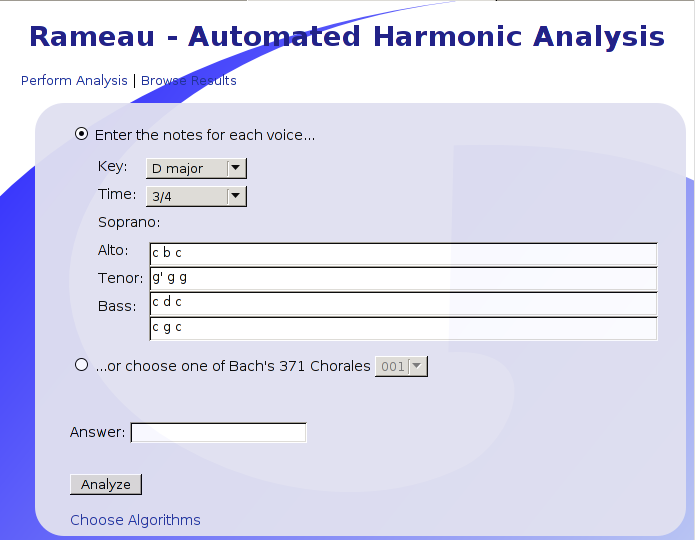
\includegraphics[scale=.5]{rameau-web}
  \caption{Rameau's web interface}
  \label{fig:rameau-web}
\end{figure*}

Rameau has nine algorithms for chord finding and four algorithms for
roman numeral analysis. Figures \ref{fig:chord-name-analysis} and
\ref{fig:roman-analysis} show the analysis result for the chord
finding and roman numeral analysis of the chorale 130 in the
Riemenschneider edition \cite{bach41:371} , respectively. Each row
shows the result for one algorithm and the last row show the expected
answer from the answer sheet. Rameau can output the result in a
text-only table or in an annotated score using LilyPond
\cite{nienhuys.ea08:lilypond} to render the score. It is noteworthy
that the decision tree, k-nearest-neighbor, and the neural net
algorithms have a 100\% accuracy in this chorale.

The answer sheet is a simple ASCII file with the chords names or the
roman numerals. The format is familiar to students of harmony classes,
the only major difference is that the numbers to indicate intervals
are separated by a dot (where they are usually piled on top of each
other in a graphical representation). For instance, a C major chord
with 7th, 9th, and 13th is represented as C7.9.13. The following is
the complete answer sheet for the chord name analysis of chorale
\#130:

\begin{verbatim}
Em D/F# G B7/F# Em B/D# C/E D7/F# [A] Em7
Am7/C Am7 D G G G/B D D Am/C Em/B [A] B 
B7 Em
\end{verbatim}

and the complete answer sheet for the roman numeral analysis is:

\begin{verbatim}
e: i V6/III III V4.3 i V6 VI6 V6.5/III
III i G: ii6.5 ii7 V I I I6 V -
e: iv6 i6.4 - V7 - i
\end{verbatim}

\begin{figure}
  \centering
  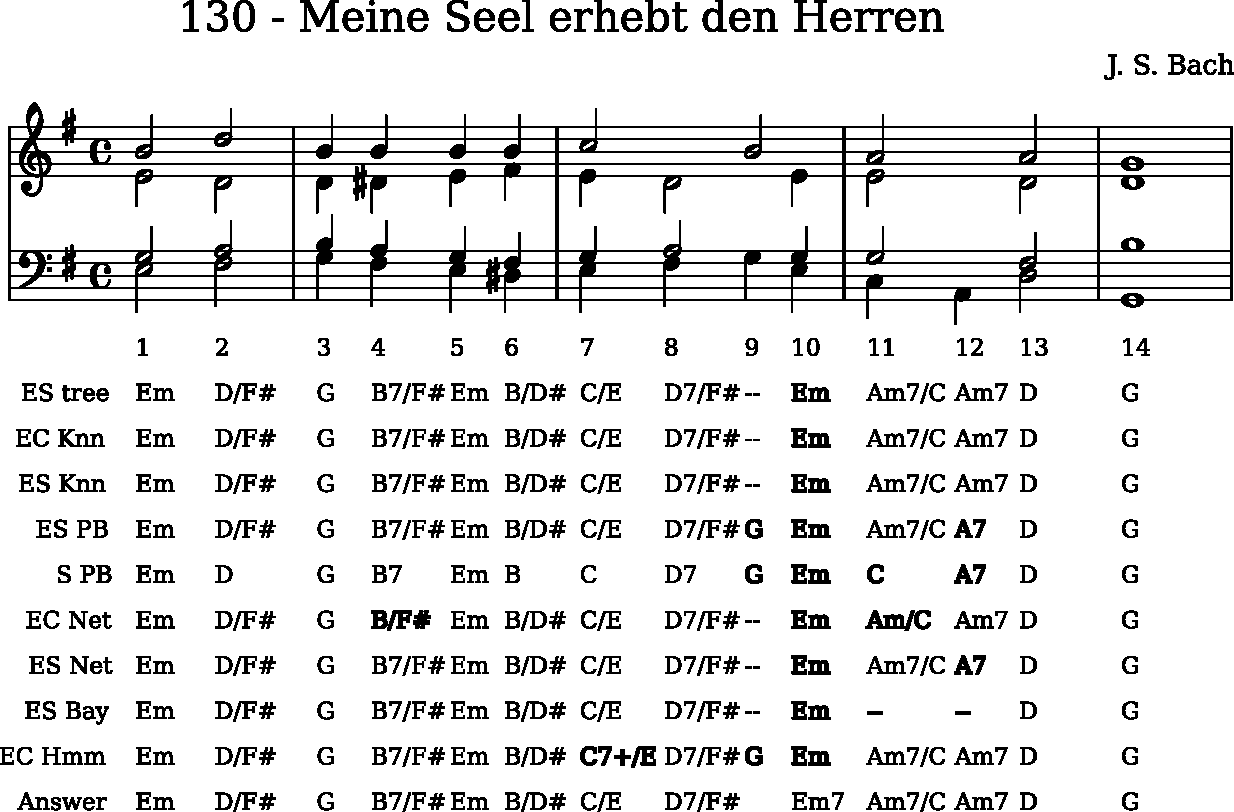
\includegraphics[scale=0.4]{analysis-130}
  \caption{Chord name analysis}
  \label{fig:chord-name-analysis}
\end{figure}
\begin{figure}
  \centering
  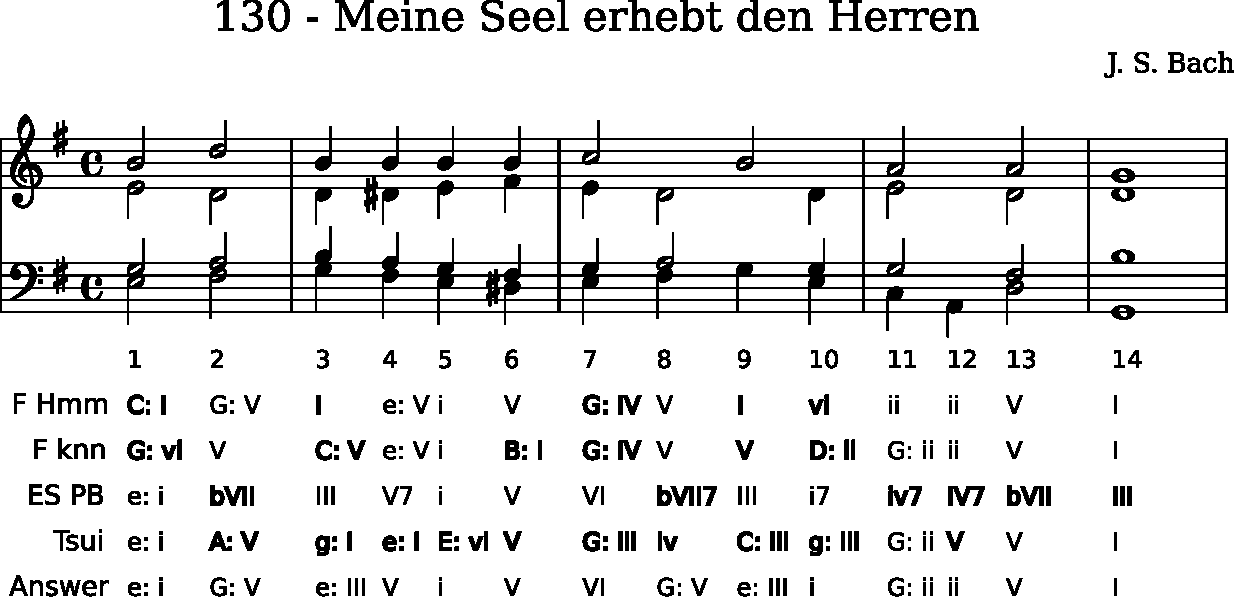
\includegraphics[scale=0.4]{analysis-functional-130}  
  \caption{Roman numeral analysis}
  \label{fig:roman-analysis}
\end{figure}


\section{Computational musicology}
\label{sec:comp-music}

We have implemented a few functions for computational musicology in
Rameau. The goal is to turn Rameau into a full framework for
computational musicology in the future.

The commands ``octaves'' and ``fifths'' show how many consecutive
octaves and fifths are in a piece and where they are. These functions
can generate lilypond scores of the passage where the octaves or
fifths happens, making it easy to visualize the results. We found, for
instance, that all consecutive octaves in Bach Chorales are in the
form unison--octave or octave--unison (see fig.
\ref{fig:oitavas-e-unissonos}), but no consecutive octaves in all
Chorales are parallel, although a few fifths are (in chorales 4, 46,
71, and 266).

\begin{figure}[!h]
  \centering
  \subfloat[Chorale \#244]{
    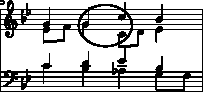
\includegraphics[scale=1]{244-oitava}
    \label{fig:244-oitava}
  }
  \qquad
  \subfloat[Chorale \#279]{
    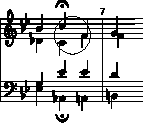
\includegraphics[scale=1]{279-oitava}
    \label{fig:279-oitava}
  }
  \qquad
  \subfloat[Chorale \#329]{
    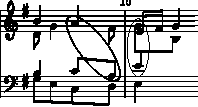
\includegraphics[scale=1]{329-oitava}
    \label{fig:329-oitava}
  }
  \caption{Consecutive octaves and unisons}
  \label{fig:oitavas-e-unissonos}
\end{figure}

The command ``chords'' list the frequency of each type of chord in a
set of chorales. For instance, we can see the type of chords in
chorale \#130 in the following list:

\begin{verbatim}
 C/F#                : 4.2% (1 of 24)
 C/D#                : 4.2% (1 of 24)
 C/E                 : 4.2% (1 of 24)
 Cm7/C               : 4.2% (1 of 24)
 Cm7                 : 4.2% (1 of 24)
 C/B                 : 4.2% (1 of 24)
 Cm/C                : 4.2% (1 of 24)
 Cm/B                : 4.2% (1 of 24)
 C7                  : 4.2% (1 of 24)
 C7/F#               : 8.3% (2 of 24)
 --                  : 8.3% (2 of 24)
 Cm                  : 16.7% (4 of 24)
 C                   : 29.2% (7 of 24)
\end{verbatim}

Not surprisingly, the major and minor triad account for the majority
of chord types. But more than 8.3\% are non-chords (marked with a
double dash), since things listed as chords like C7/F$\sharp$ and
C/D$\sharp$ are probably non-chord tones as well. With this command we
can inspect what are the most used types of sonorities, besides the
major and minor triads.

The command ``crossings'' find passages where are voice crossings. We
found that there are some kind of voice crossing in 57\% of the Bach
Chorales, although most of the crossings happen in a short period of
time (no more than two beats). There are a few interesting cases. For
instance, the alto is the lowest voice for a brief period of time in
chorale \#35 (fig. \ref{fig:035-cruzamento}) and there is a crossing
of the soprano and alto and tenor and bass at the same time in chorale
\# 290 (fig. \ref{fig:290-66-74-cruzamento}).

There are also commands to find the vocal range used in a composition,
to find melodic jumps in a voice (to analyze vocal writing, for
example), to show how the seventh of chords were resolved, and to
collect stats on how many chord progressions found in the chorales are
strong, weak, superstrong and neutral, according to Schoenberg's
theory of harmony.

\begin{figure}[!h]
  \centering
  \subfloat[Chorale \#35]{
    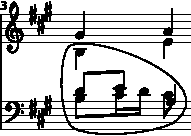
\includegraphics[scale=1]{035-16-20-cruzamento}
    \label{fig:035-cruzamento}
  }
  \subfloat[Chorale \#290]{
    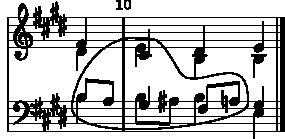
\includegraphics[scale=1]{290-66-74-cruzamento}
    \label{fig:290-66-74-cruzamento}
  }
  \caption{Voice crossing}
  \label{fig:coral-003}
\end{figure}

Finally, Rameau can analyze the final cadence of the chorales and list
then. Many commands can generate a cloud representation of its
results. The advantage of such representation is that a large amount
of data can be visualized at glance in just one picture. We can see a
cloud representation for all final cadences in the Bach Chorales in
figure \ref{fig:cadences}. From this figure it is easy to see that the
most common cadence is I ii V I, where ii can either be a minor triad
or a half-diminished seventh chord.

\begin{figure}
  \centering
  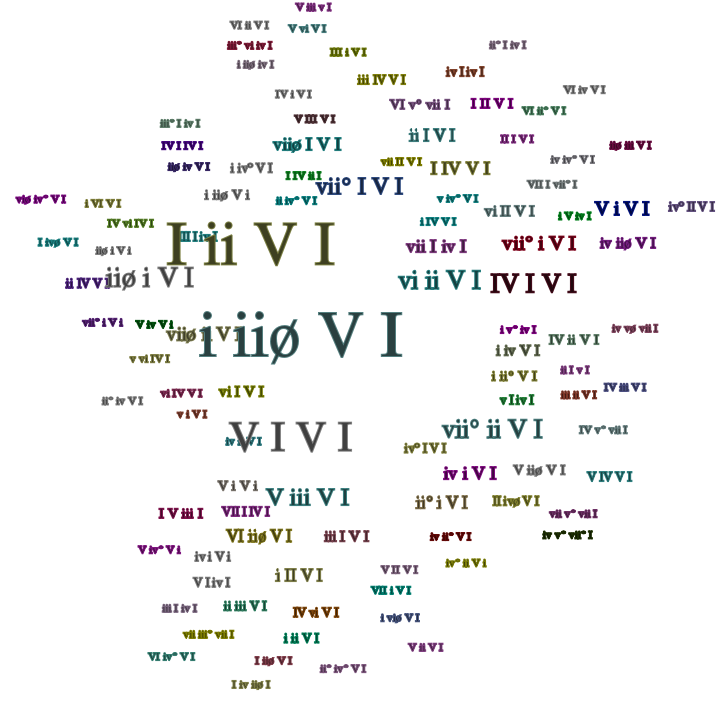
\includegraphics[scale=0.35]{cadences}
  \caption{Final cadences in Bach Chorales}
  \label{fig:cadences}
\end{figure}


\section{The functional harmonic analysis problem}
\label{sec:problem}

Roman numeral functional analysis consists, roughly, of two
activities: key finding---determining what is the tonal center of the
piece and its parts---and roman numeral function
detection---determining the tonal function of each segment of the
piece.

While this division highlights the important factors for this specific
problem it, on the other hand, ignores important sub-aspects of
harmonic analysis such as the detection of harmonically significant
segments, the disambiguation of enharmonic notes, the disambiguation
of possibly different chord types, such as telling a major chord
without a third apart from a minor chord without a third.

\subsection{Key finding}
\label{sec:key-finding}

The word ``key'', in tonal music theory, has many similar meanings,
and telling them apart is crucial when designing harmonic analysis
software. When speaking of key, a musician might speak of the key of a
piece, the key of a passage (a movement in a symphony, for example,
might have a different key from the main key in the symphony), the key
of a phrase, the key of a cadence, and even the key of a single
chord---for example, it might be argued that, for a secondary dominant
chord, its key might be said to be different from the overall key of
the surrounding passage. Clearly, there might be more or less
different scopes for the key of a song, and determining in which scope
(or scopes) to perform analysis. Another difficulty of implementing a
key finding algorithm is that there is no clear way of determining the
correctness for a key an algorithm finds for a given chord.

Another important problem involving key finding is the graphical
representation of a key that is shown to the user.

\subsection{Roman function detection}
\label{sec:roman-funct-detect}

Detecting the roman function of a segment of a piece, even after
determining its key, is also a naturally ambiguous problem. Even
defining what are the possible roman functions is not an easy problem.
For example, one might want to consider Naepolitan sixths as a roman
function, or a german augmented sixth chord, even if neither of these
is technically built from triads in the given key. Also, important
notes in a tonal function can be ommitted from the passage having that
function, and this is often done purposefully by the compose to enrich
the passage \cite{schoenberg83:theory}.


\section{The framework for functional analysis}
\label{sec:framework}

The first, and arguably most important, implementation decision when
desigining the roman numeral functional analysis part of Rameau was
the internal format for representing a complete analysis of a piece.
As described in\footnote{This reference was also removed for
  anonymity reasons, and will be present in the final paper.}, Rameau
represents a piece internally as a list of notes and, before analysis,
converts it into a list of sonorities, where a sonority is a set of
notes sounding at a given instant of time. Therefore, we chose the
format for the roman numeral functional analysis to be a list of
instantaneous analyses, where an instantaneous analysis is a snapshot
of the analysis for one sonority of a song. Due to the key granularity
problem described in section \ref{sec:key-finding}, this snapshot only
shows the most local information possible. Later on we will extend
this format to encompass notions such as the overall key of a piece or
a movement. Each such snapshot is a tuple $(K,R)$, where $K$ is the
key and $R$ is the roman numeral analysis for that sonority under key
$K$. Internally, a key is a tuple $(P_k,M_k)$, where $P_k$ is the
key's pitch and $M_k$ is the key's mode (which can be major or minor).
The roman function $R$ is also a tuple $(N,A,M_r)$, where $N$ is the
roman numeral (when applicabble), $A$ is the number of sharps (of
flats) on that numeral and $M_r$ is the roman function's mode. For
example, a minor flat seventh chord in a $D$ major key is represented
internally as $((D,major),(vii,\flat,minor)$. While this
representation has some drawbacks, such as the impossibility of
clearly marking non-harmonic passages, it is extensible and practical
for analysing simple harmonies and textures such as the Bach
chorales.

One of the goals of the Rameau project to understand and compare
previously published and new techniques for automatic harmonic
analysis. To properly compare harmonic analysis algorithms we have a
corpus of 371 Bach chorales from the Riemenschneider edition
\cite{bach41:371}, 20 of them annotated by experts with an acceptable
harmonic analysis. Rameau includes facilities to train machine
learning algorithms on these analyzed chorales and a bayesian
framework for estimating the correctness of the expert annotations and
using this estimate to derive confidence intervals for the accuracies
of the algorithms\footnote{A reference for this result was removed for
  anonymity.}. The analysis results can also be neatly typeset with
the aid of the Lilypond music typesetting program
\cite{nienhuys.ea08:lilypond}.

\section{Functional harmonic analysis algorithms}
\label{sec:algorithms}

Using the infrastructure described in section \ref{sec:framework}
Rameau currently has implementations of four different roman numeral
functional analysis; a hidden Markov model, a k-nearest neighbors
classifier, a neural network-based harmonic analyzer similar to the
one described by Tsui \cite{tsui02:harmonic}, and a trivial extension
of Pardo \& Birmingham's chord labeling algorithm
\cite{pardo.ea99:automated}.

\subsection{Hidden Markov Model}
\label{sec:hidden-markov-model}

A hidden Markov model is any probabilistic function of a Markov
chain. Using a hidden Markov model to perform roman numeral function
analysis consists of modeling the notes in a tonal piece as a
probabilistic function of the underlying harmonies, and finding these
harmonies, given the notes, using traditional hidden Markov model
algorithms. Our approach closely follows that of Raphael and Stoddard
\cite{raphael.ea03:harmonic}, and the differences will be noted here.

The underlying Markov chain is assumed to be from a pair $(K,R)$ (as
described in section \ref{sec:framework}) to another such
pair. Internally, though, this transition table is compressed assuming
some invariances (without this compression we would need around $10^9$
entries in it). The only invariance we assume is that transposing the
music to another key with the same mode should not change its
analysis. The notes found in the actual piece are assumed to be
independently and identically drawn from a distribution particular to
each possible key and roman function. This table is also compressed
assuming a transposition invariance on the key pitch. 

A good way to see how much of the underlying structure of a process is
captured by a hidden Markov model is by analysing samples from the
model. Figure \ref{fig:amostra} shows such a sample. As we can see,
the Markov model has no concept of voice leading and is quite liberal
in using non-chord tones. The line marked as ``Original'' shows the
undelying state sequence used by the hidden Markov model to generate
this piece. The line labeled ``HMM Analysis'' is an analysis of the
same piece by the HMM. It already corrects some misconceptions of the
generating model about chord structure. Finally, the line labeled
``Correct Analysis'' shows the best a human expert could do to
understand the underlying harmony of this piece. This sample also
shows an important flaw of this technique, which is the high prior
probability given to a piece that ends in an entirely different key
from the one in which it started. Perhaps some notion of a ``global''
or ``underlying'' key might improve the performance of this algorithm.

\begin{figure*}[t]
  \centering
  \includegraphics[scale=.85,trim=0cm 5cm 0cm 2.5cm]{amostra-markov}
  \caption{A sample from the hidden Markov model}
  \label{fig:amostra}
\end{figure*}

\subsection{K-Nearest Neighbors}
\label{sec:knn}

\begin{algorithm}[t]
  \SetLine
  \KwIn{$x$, an instance to be classified}
  $nearest = nil$\;
  $distance = \infty$\;
  \For{each example $e$}{
    \If{$d(e,x) < distance$}{
      $nearest = e$\;
      $distance = d(e,x)$\;
    }
  }
  \KwRet{$class(nearest)$}\;
  \caption{A nearest neighbor classifier (a knn for $k=1$).}
  \label{alg:knn}
\end{algorithm}

A tool used in machine learning for many non-trivial tasks is the
k-nearest neighbors classifier \cite{mitchell97:machine}. It works by
first representing the instances to be classified in some metric
space. Then, to classify an instance $x$, the knn algorithm chooses,
from the training data set, the set $s$ of the $k$ closest examples to
$x$ and outputs the most common class in $s$. For the case of $k=1$,
algorithm \ref{alg:knn} describes the main idea.

To apply a knn classifier in roman numeral functional analysis first
we need to choose a spatial representation of a segment of a piece,
describe an appropriate distance function, and choose a training
set. The representation we chose for Rameau is a pitch frequency array
$a$, in which, if $f*n$ on the $n$ pitches in a given sonority are
encoded (is some codification such as pitch-class or the one described
in\footnote{The reference to the original paper was removed for
  anonymity reasons.}) as having number $p$, then $a[p] = f$. When
considering surrounding context, we concatenate these arrays and, to
avoid adding too much noise in the distance function we weight them
down in proportion to the square of the distance between the
contextual sonority and the sonority being analyzed. Then, we can use
the simple euclidean distance function $d(a,b) = ||a-b||$.

\subsection{Pardo \& Birmingham's}
\label{sec:pardo--birminghams}

Pardo \& Birmingham \cite{pardo.ea99:automated} describes an algorithm
for chord labeling that has some predefined chord templates and
chooses among them the one that most closely matches the notes
sounding in a given sonority. Table \ref{tab:templates-pardo} shows
the templates used in this work.

To extend the original algorithm to perform roman numeral functional
analysis we chose not to perform any non-trivial modifications, since
those would warrant another algorithm in and of themselves. Therefore,
we simply created the key for the whole piece using the root and mode
of the first chord found by Pardo \& Birmingham's algorithm, and
thus computed the roman numeral function for all other chords in that
key. While simplistic, this approach performs almost competitively
with the hidden Markov model.

\begin{table}[h]
  \centering
  \begin{small}
    \begin{sc}
      \begin{tabular}[t]{ll} \hline
        Chord type & Notes (counting from c) \\ \hline
        Major triad & c e g \\
        Major-minor chord &  c e g b$\flat$ \\
        Minor triad & c e$\flat$ g \\
        Minor-minor chord & c $e\flat$ g b$\flat$ \\
        Fully diminished chord & c e$\flat$ g$\flat$ b$\flat\flat$ \\
        Half-diminished chord & c e$\flat$ g$\flat$ b$\flat$ \\
        Diminished triad & c e$\flat$ g$\flat$ \\
        Major-major chord & c e g b \\
        Augmented triad & c e g$\sharp$ \\
        German sixth  & c e g a$\sharp$ \\
        Italian sixth & c e a$\sharp$ \\
        French sixth & c e f$\sharp$ a$\sharp$ \\ \hline
      \end{tabular}
    \end{sc}
  \end{small}
  \caption{Templates for the Pardo \& Birmingham algorithm.}
  \label{tab:templates-pardo}
\end{table}

\section{Example analyses}
\label{sec:example-analyses}

\begin{figure*}[t]
  \centering
  \includegraphics[scale=.85,trim=0cm 4cm 0cm 1.5cm]{exemplo-01}
  \caption{An excerpt of the analysis of Bach chorale \#20.}
  \label{fig:ex01}
\end{figure*}

An example of the results of the functional analysis process is shown
is figure \ref{fig:ex01}. Each line of text under the score shows the
results for an algorithm, and the line marked ``Answer'' shows a
hand-crafted answer sheet for this passage.

\section{Conclusions and future work}
\label{sec:concl-future-work}

In this paper we presented the current status of Rameau, a framework
for automatic harmonic analysis and computational musicology. In this
framework we implemented a few algorithms for chord-labeling and roman
numeral analysis and also a few commands for computational musicology.

Also, the functions for musicology need to be further tested,
debugged, and refined. The Rameau architecture is too tied to 4-voice
part writing. We plan to address these problems in a future release of
Rameau.

While still preliminary, the current implementation of functional
harmonic analysis in Rameau is promising, and already produces useful
results. Rameau has implementations of a hidden Markov model, a
K-nearest neighbors, Pardo \& Birmingham's, and neural networks
functional harmonic analysis algorithms. Rameau is open source,
written in Common Lisp and its source code (together with our data
sets and instructions on how to compile, install and run it) is
available at \url{http://removed/for/anonymity/}.

%%% Local Variables: 
%%% mode: latex
%%% TeX-master: "icmc2009"
%%% End: 


\bibliographystyle{sbc}
\bibliography{strings-short,genos,ismir,programs,coding,harmonic-analysis,dont-have,artificial-inteligence,music-harmony-and-theory,licenses,icmc,music-scores,computational-musicology}

\end{document}
